\chapter{组织你的文本}

从这一章开始,我们将要深入 \LaTeX 编辑的各个方面,首先来看\LaTeX 文档中文本的编辑和组织,在探究中,我们会从一个一个空格、一个标点开始分析,但深入细节的同时也不要忘记整个文档的结构和组织性,要见树木更见森林。

\section{文字与符号}

\subsection{字斟句酌}

简单正文的输入没有太多特别之处,\TeX 传统上使用扩展 ASCII 字符集,较新的\TeX 引擎使用 UTF-8 编码。在接受的字符集之内,除了个别特殊符号,大部分字符可以直接录入。

\subsubsection{从字母表到单词}

在 \LaTeX 中可以从标准键盘上直接打出 26 个字母的大小写形式。当然,从字母表到单词只有一步之遥,即用空格和标点把字母分开。但事实上总免不了要遇到一些稀奇古怪的词汇或人名,试试输入下面的词:
\begin{center}
    café \quad Gödel \quad Antonín Dvořák \quad Øster Vrå \quad Kιrkağaç
\end{center}

或者这些:
\begin{center}
    χαïδεύηζ \quad КpЮковa
\end{center}

上面的例子中,前一组词是来自拉丁字母,但明显增加了许多符号;后一组则是希腊语词汇和俄语人名。我们常用的字母表包括扩展的拉丁字母、希腊字母和西里尔字母( Cyrillic alphabet ),这比标准键盘上所能直接输入的 52 个字母要多得多。不过不用担心,数以万计的汉字我们也搞定了,区区几个字母也不在话下。

解决输入超过 ASCII 码范围的字母的问题有传统和现代两类方案,先来看一下现代的方案。

现代的方案就是使用 UTF-8 编码直接输入。在 XeTeX 这样的排版引擎下, UTF-8 编码是原生的,不需要任何多余的设置:

\begin{minipage}[t]{0.45\textwidth}
    \begin{lstlisting}
    % UTF-8 编码
    café \quad Gödel \quad Antonín Dvořák

    χαïδεύηζ \quad КpЮковa
    \end{lstlisting}
\end{minipage}
\hfill
\begin{minipage}[t]{0.45\textwidth}
    \vspace{0.1cm}
    \hspace{0.5cm}

    café \quad Gödel \quad Antonín Dvořák

    χαïδεύηζ \quad КpЮковa
\end{minipage}

不过,要想正确输入、显示并输出所有这些符号,仍然不是一件简单的事。

输入特殊的字母需要计算机键盘布局或输入法的支持,例如在法语键盘中(一般可以在操作系统中设置),标准键盘 7 8 9 0 位置上的字符分别是 \verb|è _ ç à| ,这种键盘布局对需要大量录入法语的人来说特别有用。如果不方便使用特殊键盘来设置,操作系统或编辑器往往还提供了“字符映射表”一类的程序或插件,可以用鼠标选取一些字符输入;中文输入法的软键盘也可以用来输入一小部分特殊的外文字母。

显示 ASCII 以外的字母表需要编辑器使用的字体的支持。大部分西文字体都支持扩展拉丁字母,如 è 、ç ,但不是所有字体都有希腊字母和西里尔字母,即使是一些罕用的拉丁字母(如 ř 也有可能缺失。编辑器常用的等宽字体中, Windows 和 Mac 系统都预装的 Courier New , Windows 下的 Consolas 、 Lucida Sans Typewriter 等都能显示上面所列的所有字母, Linux 下常用的 Bitstream Vera Sans Mono 、 Inconsolata 则只支持到扩展拉丁字母,因此配置编辑器时也需要仔细选择。

最后但却最重要的是, \TeX 系统输出时所使用的字体,也必须要能直接显示这些字母。 \LaTeX 默认的 Computer Modern 在一个字体中只覆盖很小的字符集, XeLaTeX 下默认的 Latin Modern 字体要好得多,一般都支持到拉丁字母(这通常就足够了),但希腊、西里尔这些字体需要更换其他字体。要完整显示其他语言的字母,就必须频繁地更换不同的字体,或在 \TeX 中使用覆盖更大字符集的字体。比如为了能正确显示前面例子中的三种字母,我们在前面已经设置了 Windows 系统预装的 Times New Roman 字体。

而传统的解决方案是使用特殊的命令,给字母加上重音的标记,使用特殊字母或者整体更换字母表。

所谓重音( accents ),是指加在字母上的标记,实际包括抑音符、锐音符、抑扬符等等多种符号。 \LaTeX 支持的重音标记及其命令见表\ref{tab:zhongyin},命令名称大多取象形的符号。将重音加之于普通的拉丁字母上,可以得到一大批扩展的拉丁字母。

\begin{table}[H]
    \centering
    \caption{\LaTeX 中的重音命令,以字母 o 为例}
    \label{tab:zhongyin}
    \begin{tabular}{ccccccccccc}
        \toprule
        \`o & \verb|\`o| 
        & \qquad &
        \'o & \verb|\'o| 
        & \qquad &
        \^o & \verb|\^o| 
        & \qquad &
        \"o & \verb|\"o| \\
        \~o & \verb|\~o| 
        & \qquad &
        \=o & \verb|\=o| 
        & \qquad &
        \.o & \verb|\.o| 
        & \qquad &
        \u{o} & \verb|\u{o}| \\
        \v{o} & \verb|\v{o}| 
        & \qquad &
        \H{o} & \verb|\H{o}| 
        & \qquad &
        \t{oo} & \verb|\t{oo}| 
        & \qquad &
        \r{o} & \verb|\r{o}| \\
        \c{o} & \verb|\c{o}| 
        & \qquad &
        \d{o} & \verb|\d{o}| 
        & \qquad &
        \b{o} & \verb|\b{o}| 
        & \qquad &
         &  \\
    \bottomrule
    \end{tabular}
\end{table}

使用命令可以输入的 \LaTeX 字母,见表\ref{tab:special}。其中,\i , \j 就是字母 i , j ,只是在加上重音命令时需要去掉上面的点。 \ij,\IJ,\SS 是字母连写,在默认的字体中没有区别。

\begin{table}[H]
    \centering
    \caption{\LaTeX 中的特殊字母}
    \label{tab:special}
    \begin{tabular}{ccccccccccc}
        \toprule
        \AA & \verb|\AA| 
        & \qquad &
        \aa & \verb|\aa| 
        & \qquad &
        \AE & \verb|\AE| 
        & \qquad &
        \ae & \verb|\ae| \\
        \OE & \verb|\OE| 
        & \qquad &
        \oe & \verb|\oe| 
        & \qquad &
        \SS & \verb|\SS| 
        & \qquad &
        \ss & \verb|\ss| \\
        \IJ & \verb|\IJ| 
        & \qquad &
        \ij & \verb|\ij| 
        & \qquad &
        \L & \verb|\L| 
        & \qquad &
        \l & \verb|\l| \\
        \O & \verb|\O| 
        & \qquad &
        \o & \verb|\o| 
        & \qquad &
        \i & \verb|\i| 
        & \qquad &
        \j & \verb|\j| \\
    \bottomrule
    \end{tabular}
\end{table}

如果还要输入希腊字母和西里尔字母,默认的字体就不够用了,需要更换其他编码和字体。为此,\LaTeX 提供了 babel 宏包,可以方便地同时访问多种语言的字母表。 babel 宏包可带有一个或多个语言的可选参数,支持不同的语言,如
\begin{lstlisting}
    \usepackage[greek,english]{babel}
\end{lstlisting}
将使用英语和希腊语,其中作为最后一个参数的英语是默认语言,此时希腊语就可以用 ASCII 字符代替:
\begin{lstlisting}
    \textgreek{abcde}
\end{lstlisting}
上述代码输出 αβζδε 。需要少量俄文的西里尔字母,可以换用 OT2 编码的字体德奥。

例如:

\begin{minipage}[t]{0.45\textwidth}
    \begin{lstlisting}
% 导言区 \usepackage[OT2,OT1]{fontenc}
{\fontencoding{OT2} \selectfont ABCabc}
    \end{lstlisting}
\end{minipage}
\hfill
\begin{minipage}[t]{0.45\textwidth}
    \vspace{0.1cm}
    \hspace{0.5cm}
    {\fontencoding{OT2} \selectfont ABCabc}
\end{minipage}
如果排版全文是俄文的文章,也可以用 \verb|russian| 参数使用 \verb|babel| 宏包,不过输入时就不使用 ASCII 码,而使用俄文专用的编码。由于这些语言很少用,这里不做更多说明。

使用 pdfTeX 这样的传统排版引擎也可以使用 UTF-8 编码输入文字,此时需要使用 inputenc 宏包并选用 \verb|utf8| 选项,它会将 UTF-8 的输入编码自动转换为当前字体编码所对应的符号,字体编码的设置仍然与原来一样,如:
\begin{lstlisting}
    % coding: utf-8
    % pdflatex 命令编译
    \documentclass{article}
    \usepackage[OT2,OT1]{fontenc}
    \usepackage[utf8]{inputenc}
    \begin{document}
    café \quad Gödel
    {\fontencoding{OT2} \selectfont КpЮковa}
    \end{document}
\end{lstlisting}

\LaTeX 在排版中会将单词中的一些字母连写成为一个符号,即连字 ( ligature )。连字的有无和多少一般是由使用的字体决定的,在默认的 Computer Modern 和 Latin Modern 字体中,小写字母组合 \verb|ff,fi,fl,ffi,ffl| 都有连字:

\begin{minipage}[t]{0.45\textwidth}
    \begin{lstlisting}
    differ find flight difficult ruffle 
    \end{lstlisting}
\end{minipage}
\hfill
\begin{minipage}[c]{0.45\textwidth}
    \hspace{0.5cm}
    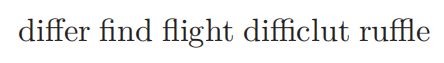
\includegraphics[width=0.6\textwidth]{连字1.png}
\end{minipage}

本书中主要使用的 Times 字体则只有 \verb|fi| 和 \verb|fl| 的连字 ( fi,fl),而一些专业字体可能用的更多:

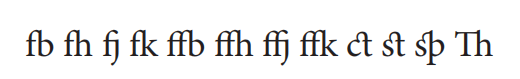
\includegraphics[width=0.3\textwidth]{连字2.png}

偶尔出于意义或美观的考虑,需要取消连字。此时可以借用\verb|\/|命令。

\begin{minipage}[t]{0.45\textwidth}
    \begin{lstlisting}
    fleet f\/leet
    \end{lstlisting}
\end{minipage}
\hfill
\begin{minipage}[b]{0.45\textwidth}
    \hspace{0.5cm}

    fleet f\/leet
\end{minipage}

使用 XeLaTeX 引擎, OpenType 字体时,可以方便地使用 fontspec 宏包的 \verb|Ligature| 字体选项选择连字的有无和程度。

\subsubsection{正确使用标点}

在键盘上,可以直接使用的符号有 16 种:

, \quad . \quad ; \quad : \quad ! \quad ? \quad ` \quad ' \quad ( \quad ) \quad [ \quad ] \quad - \quad /  \quad * \quad @

标点\ ,\ .\ ;\ :\ !\ ?\ 用来分隔句子或部分句子,在每个标点之后应该加上空格,以保证正确的距离和换行。在特殊情况下,这些标点有空格还有一些更微妙的关系。

引号在 \LaTeX 中用 \verb|`|和 \verb|'| 两个符号表示。单引号就用一遍,双引号用两遍。如果遇到单引号和双引号连续出现的情形,则在中间用 \verb|\,|命令分开:

\begin{minipage}[t]{0.45\textwidth}
    \begin{lstlisting}
    ``\,`A' or `B?' \,'' he asked.
    \end{lstlisting}
\end{minipage}
\hfill
\begin{minipage}[t]{0.45\textwidth}
    \vspace{0.1cm}
    \hspace{0.5cm}
    ``\,`A' or `B?' \,'' he asked.
\end{minipage}
这里\verb|\,| 命令产生很小的间距,注意\LaTeX 并不会忽略以符号命名的宏前后的空格,所以在它前后都不要加多余的空格。符号\verb|'| 同时也是表示所有格和省字的撇号 ( apostrophe ,如 ``It's Knuth's book'' )。

引号和括号通常要在前后加空格分割单词。逗号、句号等标点何时放在引号和括号内,何时放在引号和括号外,可参见英文写作的格式指导。

除了在数学模式中表示减号,符号 - 在\LaTeX 正文中也有多种用途:单独使用时它是连字符( hyphen );两个连用( -- ),是 en dash ,用来表示数字范围;三个连用 ( --- ),是 em dash ,即破折号:

\begin{minipage}[t]{0.45\textwidth}
    \begin{lstlisting}
        
    An inter-word dash or , hyphen, as in X-ray.

    A medium dash for number ranges, like 1--2.

    A punctuation dash --- like this.
    \end{lstlisting}
\end{minipage}
\hfill
\begin{minipage}[t]{0.45\textwidth}
    \vspace{0.1cm}
    \hspace{0.5cm}

    An inter-word dash or , hyphen, as in X-ray.

    A medium dash for number ranges, like 1--2.

    A punctuation dash --- like this.
\end{minipage}

不过,按中文写作习惯,表示数字范围也常使用符号 $\sim$ (\verb|$\sim$|) ,有时也用汉字的全角破折号或半个汉字破折号。

西文的省略号( ellipsis )使用\verb|\ldots| 或 \verb|\dots| 命令产生,相比直接输入三个句号,它所拉开的距离要合理些:

\begin{minipage}[t]{0.45\textwidth}
    \begin{lstlisting}
    Good: One, two, three \ldots

    Bad: One, two, three...
    \end{lstlisting}
\end{minipage}
\hfill
\begin{minipage}[t]{0.45\textwidth}
    \vspace{0.1cm}
    \hspace{0.5cm}

    Good: One, two, three \ldots

    Bad: One, two, three...
\end{minipage}

\verb|\ldots| 和 \verb|\dots| 命令在正文中是等价的,它们会在每个点后面增加一个小的间距,因而直接在 \verb|\ldots| 后面再加逗号、句号、叹号等标号,也能得到正确的间距。西文省略号的用法在不同的格式手册中往往有详细规定,通常在句中使用时,前后都要加空格,而在句末使用则应该使用 4 个点。这是因为 \verb|\ldots| 的后面也有间距,所以使用\verb|H\ldots.| 能得到正确的 “ H\ldots. ”,但直接使用 \verb|H \ldots\ H| 却将得到错误的间距 “ H \ldots\ H ”(后一个间距比前面大 )。解决的办法是把省略号放进数学模式:

\begin{minipage}[t]{0.45\textwidth}
    \begin{lstlisting}
    She $\ldots$ she got it.

    I've no idea\ldots.
    \end{lstlisting}
\end{minipage}
\hfill
\begin{minipage}[t]{0.45\textwidth}
    \vspace{0.1cm}
    \hspace{0.5cm}

    She $\ldots$ she got it.

    I've no idea\ldots.
\end{minipage}

标准键盘上不能直接录入的标点符号有10个,它们占据了主键盘上面一大排的一大半:

\~{} \quad \# \quad \$ \quad \% \quad \^{} \quad \& \quad \{ \quad \} \quad \_ \quad \textbackslash 

他们都有特殊作用,其中的许多我们已经熟知:数学模式符号 \$ 、注释符号 \% 、上标 \^{} 、分组 \{\} 、宏命令 \textbackslash,只有个别例外:

\begin{minipage}[t]{0.45\textwidth}
    \begin{lstlisting}[language = java]
    \~{} \quad \# \quad \$ \quad \% 
    \quad \^{} \quad \& \quad \{ \quad \} 
    \quad \_ \quad \textbackslash 
    \end{lstlisting}
\end{minipage}
\hfill
\begin{minipage}[t]{0.45\textwidth}
    \vspace{0.1cm}
    \hspace{0.5cm}

    \~{} \quad \# \quad \$ \quad \% \quad \^{} \quad \& \quad \{ \quad \} \quad \_ \quad \textbackslash 
\end{minipage}

可以用没有字母的重音\verb|\~{}| 和 \verb|\^{}| 输出 \~{} 和 \^{} ,但这两个符号一般不直接在普通正文中出现,而出现其他地方:可以是重音符号;可以出现在程序代码中;此外还有一个数学符号 $\sim$。

符号

| \quad < \quad > \quad + \quad =

虽然可以接受,但它们一般用在数学公式中,其文本形式的效果不好或有错,一般不直接使用它们。键盘上的双引号 \verb|"| 一般也极少使用在正文中,而常被另外定义移作他用。

中文使用的标点与西文标点不同 中文写作使用全角标点:

\begin{table}[H]
    \centering
    \begin{tabular}{ccccccccccc}
        句号 & 。或\ . & &
        逗号 & , & &
        顿号 & 、& &
        分号 & ; \\
        冒号 & : &&
        问号 & ? &&
        感叹号 & ! &&
        间隔号 & · \\ 
        单引号 & ‘ \quad ’ &&
        双引号 & “ \quad ” &&
        单书名号 & <\quad  > &&
        双书名号 & 《\quad 》 \\
        括号 & () [] ﹝﹞ &&
        省略号 & …… && 
        破折号 & —— 
    \end{tabular}
\end{table}

在计算机中使用中文输入法录入全角标点通常是很直接的。特别需要说明的是破折号( —— )和 省略号 (……),它们都占两个中文字符,在大部分输入法中可以使用 \verb|Shift+-| 和 \verb|Shift+6| 得到。

在科技文章中,为与数字、字母区分,中文的句号一般也用一个圆点表示,此时应该使用全角的“.” 而非混用西文句点。这个标点在大部分中文输入法下可能不易输入,可以先统一使用句号“。”,最后统一替换。

也有一种科技文章的写作风格,是中文与西文统一使用西文的标点,只有顿号、破折号和省略号仍用中文标点。但这样可能造成标点大小、位置与汉字对不准,以及字体风格的不统一,应该小心使用。

\LaTeX 并不会自动处理好汉字标点的宽度和间距,甚至不能保证标点的禁则(如句号不允许出现在一行的开始)。使用 XeTeX 作为排版引擎时,中文标点一般是由 xeCJK 宏包控制的。 xeCJK 提供了多种标点格式,默认是全角式,即所有标点占一个汉字宽度,只有在行末或个别标点之间进行标点挤压。还支持其他一些标点格式,可以使用\verb|\punctstyle| 命令修改:

\begin{center}
    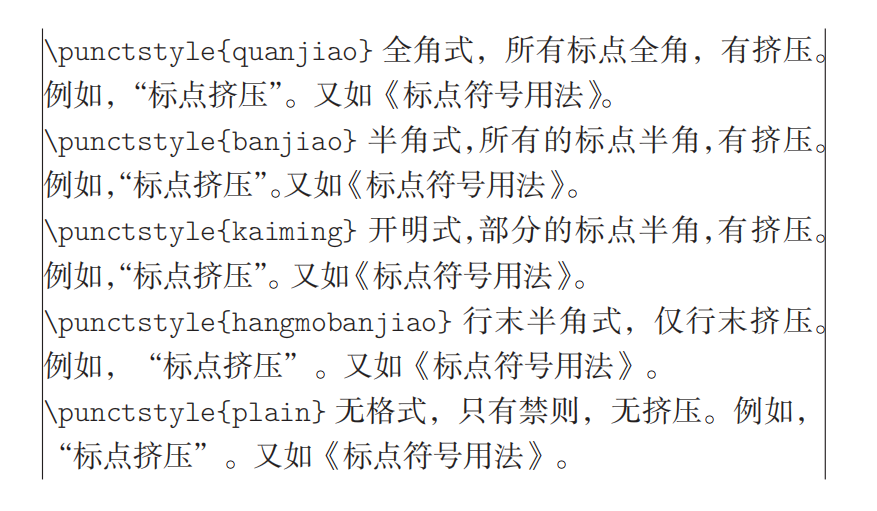
\includegraphics[width=0.6\textwidth]{标点形式.png} \centering
\end{center}

\subsubsection{看不见的字符——空格与换行}

文本中的空格起分隔单词的作用,任意多个空格的功能与一个空格相同;只有字符后面的空格是有效的,每行最前面的空格则被忽略,这样有利于复杂代码的对齐;单个换行也被看成一个空格。例如(我们仍然用 \lstinline[showspaces=true]{ } 表示空格:

\begin{minipage}[t]{0.45\textwidth}
    \begin{lstlisting}[showspaces=true]
This is     a short
sentence.  This is
             another.
\end{lstlisting}
\end{minipage}
\hfill
\begin{minipage}[c]{0.45\textwidth}
This is     a short
sentence.  This is
             another.
\end{minipage}

以字母命名的宏,后面空格会被忽略。如果需要再命令后面使用空格,可以使用\lstinline[showspaces=true]{\ },它表示两个普通字母间的空格距离;也可以在命令后加一个空白的分组\verb|{}|,有时也可以把命令用一个分组包裹起来:

\begin{minipage}[t]{0.45\textwidth}
\begin{lstlisting}[showspaces=true]
Happy \TeX ing. Happy \TeX\ ing.
Happy  \TeX{} ing. Happy {\TeX} ing.
\end{lstlisting}
\end{minipage}
\hfill
\begin{minipage}[t]{0.45\textwidth}
Happy \TeX ing. Happy \TeX\ ing.

Happy  \TeX{} ing. Happy {\TeX} ing.
\end{minipage}

有一种不可打断的空格,在\TeX 中称为带子( ties ),用\verb|~| 表示。 \TeX 禁止在这种空格之间分行,因而可以用来表示一些不宜分开的情况,例如:
\begin{lstlisting}
    Question~1              % 名称与编号间
    Donald~E. Knuth         % 教名之间,但姓可以断行
    Mr.~Knuth               % 称谓缩写与名字间
    function~$f(x)$         % 名字后面的短公式
    1,~2,and~3              % 序列的部分符号间
\end{lstlisting}

西文的逗号、句号、分号等标点后面应该加空格,这不仅能保证正确的间距,也能保证正确的换行。这是因为标点后如果没有空格,就不能换行。\LaTeX 在西文句末(包括句号\verb|.|问号\verb|?|和叹号\verb|!|)后面使用的距离会比单词间的距离大些,这在上面的例子中已经可以看到。更确切地说,\LaTeX 会把大写字母后的点看作是缩写标记,把小写后面的点看作是句子结束,并对它们使用不同的间距;但偶尔也有大写字母结束的句子,或小写字母的缩写,这就必须明确地告诉 \LaTeX 使用普通单词间的空格 \lstinline[showspaces=true]{\ } ,或用\verb|\@|,指明\verb|.| 是大写字母后的句末。例如:

\begin{minipage}[t]{0.45\textwidth}
\begin{lstlisting}[showspaces=true]
A sentence. And another.

U.S.A. means United States Army?

Tinker et al.\ made the double play.

Roman number XII\@. Yes.
\end{lstlisting}
\end{minipage}
\hfill
\begin{minipage}[t]{0.45\textwidth}
A sentence. And another.

U.S.A. means United States Army?

Tinker et al.\ made the double play.

Roman number XII\@. Yes.
\end{minipage}
有时也需要整体禁止这种在标点后的不同的间距,法语排版的习惯就是如此。此时可以使用\verb|\frenchspacing| 命令来禁止标点后的额外间距。

汉字后的空格会被忽略。使用 xelatex 编译中文文档时,汉字和其他内容之间如果没有空格, xeCJK 宏包会自动添加:

\begin{minipage}[t]{0.45\textwidth}
\begin{lstlisting}[showspaces=true]
中文和English的混排效果并不依赖 space 的有无 
\end{lstlisting}
\end{minipage}
\hfill
\begin{minipage}[t]{0.45\textwidth}
    中文和English的混排效果并不依赖 space 的有无
\end{minipage}

个别时候需要忽略汉字与其它内容之间由 xeCJK 自动产生的空格,这时可以把汉字放进一个盒子里面:

\begin{minipage}[t]{0.45\textwidth}
\begin{lstlisting}[showspaces=true]
\mbox{条目}a 不同于条目b
\end{lstlisting}
\end{minipage}
\hfill
\begin{minipage}[t]{0.45\textwidth}
\mbox{条目}a 不同于条目b
\end{minipage}

还有时需要完全禁用汉字与其他内容之间的空格,这时可以使用\verb|\CJKsetecglue| 手工设置汉字与其他内容之间的内容为空\footnote{好像现在这个方法已经失效}(默认是一个空格):

\begin{minipage}[t]{0.45\textwidth}
\begin{lstlisting}
\CKJsetecglue{}
汉字word
\end{lstlisting}
\end{minipage}
\hfill
\begin{minipage}[t]{0.45\textwidth}
\mbox{汉字}word 
\end{minipage}

在空格之中,最神奇的一种可能就是被称为幻影( phantom )的空格。幻影命令\verb|\phantom| 有一个参数,作用是产生与参数内容一样大小的空盒子,没有内容,就像是参数的一个幻影一样。偶尔可以使用幻影完成一些特殊的占位和对齐效果:

\begin{minipage}[t]{0.45\textwidth}
\begin{lstlisting}
    幻影\phantom{参数}速速隐形

    幻影参数速速显形
\end{lstlisting}
\end{minipage}
\hfill
\begin{minipage}[t]{0.45\textwidth}
    幻影\phantom{参数}速速隐形

    幻影参数速速显形
\end{minipage}

类似地有\verb|\hphantom| 和 \verb|\vphantom| ,分别表示水平方向和垂直方向的幻影(在另一个方向为零)。

空行,即用连续两个换行表示分段,段与段之间会自动得到适合的缩进。任意多个空行有一个空行的效果相同。

分段也可用用\verb|\par| 命令生成,这种方法一般只在命令或环境定义的内部使用,而普通行文中不宜出现。与连续的空行类似,连续的\verb|\par| 命令也只产生一次分段效果。

除了分段,也可以让\LaTeX 直接另起一行,并不分段。优良中相关的命令:\verb|\\| 命令直接另起一行,上一行保持原来的样子;而\verb|\linebreak| 则指定一行的断点,上一行仍按照一行散开对齐:

\begin{minipage}[t]{0.45\textwidth}
\begin{lstlisting}
    这是一行文字\\另一行

    这是一行文字\linebreak 另一行
\end{lstlisting}
\end{minipage}
\hfill
\begin{minipage}[t]{0.45\textwidth}
    这是一行文字 \\ 另一行

    这是一行文字\linebreak 另一行
\end{minipage}

\verb|\\| 一般用于特殊的环境中,如排版诗歌的 \verb|verse| 环境,特别是在对齐、表格和数学公式中使用广泛,但很少用在普通正文的行文中;\verb|\linebreak| 命令则用于对个别不适合分行的手工精细调整上。为了完成精细调整分行的功能,\verb|\linebreak| 可以带一个从 0 到 4 的可选参数,表示允许断行的程度, 0 表示不允许断行, 默认的 4 表示必须断行。类似地,也有一个\verb|\nolinebreak| 命令,只是参数意义与\verb|\linebreak| 相反。注意在正常的行文中,这两个命令都不会被用到。

\verb|\\| 命令可以带一个可选的长度参数,表示换行后增加的额外垂直间距。如\verb|\\[2cm]| 。因此必须注意在命令\verb|\\| 后面如果确实需要使用方括号(即使括号在下一行),则应该在\verb|\\| 后面加空的分组以示分隔,否则会发生错误,这种情况在数学公式中非常常见:

\begin{minipage}[t]{0.45\textwidth}
\begin{lstlisting}
\begin{align*}
[2 - (3+5)] \times 7 & = 42 \\ {}
[2 + (3-5)] \times 7 & = 0
\end{align*}
\end{lstlisting}
\end{minipage}
\hfill
\begin{minipage}[t]{0.45\textwidth}
\begin{align*}
[2 - (3+5)] \times 7 & = 42 \\ {}
[2 + (3-5)] \times 7 & = 0
\end{align*}    
\end{minipage}

